\documentclass[11pt]{article}

\usepackage{working-paper}
\usepackage{amsmath,amsthm}
\usepackage{booktabs}
\usepackage{graphicx}
\usepackage{adjustbox}
\usepackage{xurl}
\setlength{\emergencystretch}{2em}
\graphicspath{{../figs/}}

\newcommand{\simNReps}{400}
\newcommand{\simDim}{64}
\newcommand{\simPairs}{80}
\newcommand{\simObs}{600}
\newcommand{\simTrueTheta}{1.50}
\newcommand{\simCleanCosMean}{0.99}
\newcommand{\simCleanSplitMean}{0.97}
\newcommand{\simNoisyROne}{0.57}
\newcommand{\simNoisySplitPca}{0.97}
\newcommand{\simNoisyCosPca}{0.07}
\newcommand{\simNoisyCosMean}{0.97}
\newcommand{\simNoisySplitMean}{0.90}
\newcommand{\simDispROne}{0.11}
\newcommand{\simDispSplitMean}{0.19}
\newcommand{\simDispSplitPca}{0.21}
\newcommand{\simOlsBias}{+0.773}
\newcommand{\simOlsRmse}{0.776}
\newcommand{\simPcaBias}{-1.458}
\newcommand{\simMeanBias}{+0.004}
\newcommand{\simMeanRmse}{0.047}
\newcommand{\simMeanCov}{93.2}
\newcommand{\simMeanRTwo}{0.43}
\newcommand{\simNaiveBias}{+1547.2}
\newcommand{\simNaiveRmse}{46245.7}
\newcommand{\simNaiveRTwo}{1.00}
\newcommand{\simOblBias}{-0.002}
\newcommand{\simOblRmse}{0.037}
\newcommand{\simOblCov}{93.8}
\newcommand{\simOblRTwo}{0.16}

\newcommand{\empNWiki}{4,353}
\newcommand{\empNSe}{6,603}
\newcommand{\empPolROne}{0.37}
\newcommand{\empPolSplit}{0.92}
\newcommand{\empPolOod}{0.70}
\newcommand{\empUrgSplit}{0.98}
\newcommand{\empUrgOod}{0.83}
\newcommand{\empPluSplit}{0.84}
\newcommand{\empRndROne}{0.37}
\newcommand{\empRndSplit}{0.14}
\newcommand{\empRndOod}{0.13}
\newcommand{\empCosPolUrg}{0.11}
\newcommand{\empWikiOls}{+0.275}
\newcommand{\empWikiDml}{+0.202}
\newcommand{\empWikiDmlSe}{0.020}
\newcommand{\empWikiRTwo}{0.64}
\newcommand{\empSeOls}{+0.014}
\newcommand{\empSeOlsSe}{0.013}
\newcommand{\empSeDml}{+0.065}
\newcommand{\empSeDmlSe}{0.020}
\newcommand{\empSeRTwo}{0.62}
\newcommand{\empWikiObl}{+0.203}
\newcommand{\empSeObl}{+0.066}
\newcommand{\empWikiNav}{+1.900}
\newcommand{\empSeNav}{+0.853}
\newcommand{\empWikiProbe}{+0.420}
\newcommand{\empWikiProbeSe}{0.025}
\newcommand{\empWikiProbeRTwo}{0.76}
\newcommand{\empSeProbe}{+0.319}
\newcommand{\empSeProbeRTwo}{0.74}
\newcommand{\empWikiNoKwPct}{82}
\newcommand{\empWikiNoKwN}{3,578}
\newcommand{\empSeNoKwPct}{86}
\newcommand{\empSeNoKwN}{5,647}
\newcommand{\empWikiImp}{+0.154}
\newcommand{\empWikiImpSe}{0.021}
\newcommand{\empSeImp}{+0.060}
\newcommand{\empSeImpSe}{0.022}
\newcommand{\empPcPairAcc}{38.3}
\newcommand{\empPcDomR}{0.39}
\newcommand{\empRLenOurs}{0.04}
\newcommand{\empRLenProbeLo}{0.11}
\newcommand{\empRLenProbeHi}{0.13}
\newcommand{\empWikiPluOls}{+0.041}
\newcommand{\empWikiPluOlsSe}{0.015}
\newcommand{\empWikiPluDml}{-0.009}
\newcommand{\empSePluDml}{-0.002}
\newcommand{\empWikiPluDmlSe}{0.019}
\newcommand{\empWikiRandOls}{70}
\newcommand{\empSeRandOls}{50}
\newcommand{\empWikiRandDml}{5}
\newcommand{\empSeRandDml}{5}


\newcommand{\TableStyle}{\small\setlength{\tabcolsep}{5pt}\renewcommand{\arraystretch}{1.05}}

\newtheorem{proposition}{Proposition}
\newtheorem{assumption}{Assumption}

\title{One Concept at a Time:\\
Subspace-Constrained Causal Inference for High-Dimensional Treatments}
\author{Gaurav Sood}
\date{March 2026}

\begin{document}
\maketitle

\begin{abstract}
\noindent When treatments are complex objects such as texts, images, or audio, researchers rarely want the causal effect of the raw object. They want the causal effect of a single human-interpretable attribute, such as politeness, threat, or formality, holding all other attributes fixed. Surface edits routinely change multiple correlated attributes at once, and latent factors discovered from observational corpora blend target concepts with background confounders. We separate concept geometry from causal estimation in two stages using a frozen pretrained representation $h(T) \in \mathbb{R}^d$. In Stage~1, external contrastive minimal pairs define a low-dimensional concept subspace $U_k \in \mathbb{R}^{d \times k}$. We show that uncentered second-moment singular value decomposition conflates the mean concept shift with zero-mean nuisance edit noise, so one-dimensional concepts should be estimated by the normalized mean shift while centered covariance components diagnose context heterogeneity. Pre-outcome checks on variance concentration, split-half stability, and cross-domain transfer allow researchers to reject ill-posed concepts before viewing outcomes. In Stage~2, we decompose representations into concept coordinates and their orthogonal complement, using oblique pseudoinverse projections when multiple concepts are non-orthogonal, and estimate causal effects via activation steering (with round-trip decoding checks) or cross-fitted double/debiased machine learning (DML). When minimal pairs come from an external sample, DML inference for the subspace-conditional estimand is exact conditional on $\hat{U}_k$, while recovery of a population subspace parameter follows a Davis--Kahan eigengap rate. Applying the method with a lightweight 22M-parameter encoder (\texttt{all-MiniLM-L6-v2}) to \empNWiki{} Wikipedia requests and \empNSe{} Stack Exchange requests recovers politeness effects of \empWikiDml{} (SE \empWikiDmlSe) and \empSeDml{} (SE \empSeDmlSe) SD per SD, passes negative-control and permutation placebos, and cuts random-direction false positives from \empWikiRandOls\% and \empSeRandOls\% under unadjusted OLS to \empWikiRandDml\% under DML.
\end{abstract}

\section{Introduction}

Suppose a political scientist wants to measure how politeness in constituent emails affects legislative responsiveness, or how assertive wording in a policy appeal changes public support. Respondents encounter a full text $T$. The scientific hypothesis, however, is not about one string of words. It is about an abstract concept $C$ carried by the text while all other bundled attributes $W$ remain fixed.

Isolating $C$ from $W$ is difficult because surface edits bundle attributes together. Rewriting ``Send me the budget spreadsheet by 5 PM'' as ``Would you mind sending over the budget spreadsheet by 5 PM if your schedule permits?'' adds politeness markers, but it also softens deadline urgency, lengthens the message, and shifts perceived status. Unsupervised topic models and latent-treatment discovery methods avoid hand-coding edits, yet factors extracted from observational corpora routinely merge target concepts with correlated topics and sender traits \citep{fong2016discovery,egami2022make,fong2023causal}. Supervised classifiers and linear probes trained on labeled observational texts suffer the same contamination: weights chosen to predict labels in one domain absorb spurious domain correlates \citep{veitch2020adapting,ravfogel2020null,belinkov2022probing}.

Meanwhile, representation engineering has shown that pretrained neural models often encode high-level semantic and stylistic concepts along low-dimensional linear subspaces in intermediate activation vectors $h(T) \in \mathbb{R}^d$ \citep{alain2016understanding,meng2022locating,turner2023activation,zou2023representation,park2023linear}. Adding a steering vector during a forward pass shifts generated text along concept $C$ \citep{li2023inference,rimsky2024steering}. That literature treats linear directions as engineering heuristics for model control, without formal causal estimands, confounding adjustment, or criteria for rejecting concepts that do not form clean linear subspaces.

We turn linear representation geometry into a falsifiable, two-stage causal inference design. Stage~1 uses external contrastive minimal pairs and a frozen pretrained encoder, without viewing outcomes $Y$, to estimate a low-dimensional concept subspace $U_k \in \mathbb{R}^{d \times k}$ and test whether the concept concentrates along a stable, cross-domain linear direction. If the diagnostics fail, the researcher stops before outcome analysis. When Stage~1 passes, Stage~2 decomposes every text representation into low-dimensional concept coordinates $Z_i$ and a high-dimensional orthogonal complement $R_i$, then estimates causal effects either by experimental steering (with round-trip decoding checks) or by cross-fitted double/debiased machine learning \citep[DML;][]{robinson1988root,chernozhukov2018double}.

Developing this pipeline uncovers four analytical pitfalls that break naive implementations. First, extracting a concept direction from the top eigenvector of the uncentered second-moment matrix $S = \frac{1}{m}DD^\top$ conflates the systematic mean shift $\bar{\Delta h}$ with high-variance zero-mean edit noise; using the normalized mean shift averages out zero-mean nuisance edits at rate $O_P(m^{-1/2})$. Second, when researchers stack $k$ distinct concept vectors estimated from separate minimal-pair sets, the columns of $U_k$ are generally non-orthogonal ($U_k^\top U_k \neq I_k$). Applying the single-concept orthogonal residual $(I_d - U_k U_k^\top)h_i$ leaks concept signal into the control residual and makes multi-concept DML explode; valid estimation requires the oblique Moore--Penrose pseudoinverse projection. Third, Euclidean orthogonality ($U_k^\top R_i = 0$) does not imply statistical independence in anisotropic neural representations ($\mathrm{Cov}(h(T)) \neq \sigma^2 I_d$), so observational studies must control for a reduced-rank orthonormal basis of $R_i$ and report the first-stage overlap diagnostic $R^2(Z \mid R)$. Fourth, when minimal pairs come from an external sample independent of the outcome study, DML standard errors are exact conditional on $\hat{U}_k$ for the locked-subspace estimand, while recovery of a latent population subspace parameter is governed by a Davis--Kahan eigengap bound \citep{davis1970rotation}.

Monte Carlo simulations and an empirical application confirm these results. Using a lightweight 22M-parameter encoder (\texttt{all-MiniLM-L6-v2}) on \empNWiki{} Wikipedia talk-page requests and \empNSe{} Stack Exchange requests from the Stanford Politeness Corpora \citep{danescu2013computational}, external minimal pairs pass Stage~1 with split-half stability \empPolSplit{} and cross-domain transfer \empPolOod, whereas sign-flipped placebos are rejected (\empRndSplit) despite identical uncentered $R_1^2$. In Stage~2, 5-fold DML trims upward confounding on Wikipedia (\empWikiOls{} under OLS to \empWikiDml{} under DML) and rescues a topic-suppressed effect on Stack Exchange (\empSeOls{} under OLS to \empSeDml{} under DML). On the \empWikiNoKwPct\% to \empSeNoKwPct\% of requests containing zero explicit politeness keywords, where lexical proxies are undefined, our subspace DML still recovers implicit politeness effects (\empWikiImp{} and \empSeImp). Across random orthogonal directions, unadjusted OLS falsely rejects \empWikiRandOls\% on Wikipedia and \empSeRandOls\% on Stack Exchange at the 5\% level, while DML achieves exact \empWikiRandDml\% nominal size on both corpora and returns null estimates (\empWikiPluDml{} and \empSePluDml) on a negative-control grammatical concept.

\section{High-Dimensional Treatments and Representation Geometry}

Let $\mathcal{T}$ denote the space of surface objects such as texts, images, or audio clips. Each unit $i \in \{1, \dots, n\}$ in an empirical study is exposed to an object $T_i \in \mathcal{T}$ and produces a scalar outcome $Y_i \in \mathbb{R}$. Conceptually, each object carries a target attribute $C$ (such as politeness or urgency) alongside a high-dimensional bundle of non-target attributes $W$ (topic, factual claims, length, syntax, and domain vocabulary).

We treat a frozen pretrained foundation model as a deterministic measurement map $h : \mathcal{T} \to \mathbb{R}^d$, extracted from a fixed intermediate layer and token aggregation rule. Crucially, the parameters of $h(\cdot)$ are fixed before the study and never tuned on outcome data $Y$. Independent of the outcome sample $\mathcal{D}_{\mathrm{obs}} = \{(T_i, Y_i)\}_{i=1}^n$, the researcher collects an external set of $m$ contrastive minimal pairs $\mathcal{D}_{\mathrm{pairs}} = \{(T_j^-, T_j^+)\}_{j=1}^m$, where $T_j^+$ edits $T_j^-$ to increase concept $C$ while holding $W$ as constant as possible.

\subsection{Representation Sufficiency and Causal Estimands}

In studies with human evaluators, respondents react to the rendered object $T$, generating potential outcomes $Y_i(T)$. Defining a ceteris paribus intervention in representation space requires linking $Y_i(T)$ to $h(T)$.

\begin{assumption}[Representation Sufficiency for Potential Outcomes]\label{ass:rep_sufficiency}
For any two surface objects $T, T' \in \mathcal{T}$, if $h(T) = h(T')$, then $Y_i(T) = Y_i(T')$ almost surely. Given a full-rank basis $U_k \in \mathbb{R}^{d \times k}$ spanning a concept subspace $\mathcal{S}_C$ with projection $P_{U_k}$, every representation decomposes uniquely as $h(T) = U_k z + r$ with $U_k^\top r = 0$, inducing a well-defined potential outcome function $Y_i(z, r)$ such that $Y_i(T) = Y_i(z, r)$.
\end{assumption}

Assumption~\ref{ass:rep_sufficiency} is load-bearing because human readers see surface text rather than hidden vectors. If pooling at layer $\ell$ discards a punctuation cue or lexical detail that affects human responses, then holding $r$ fixed in $\mathbb{R}^d$ fails to hold all outcome-relevant background features fixed. Selecting a rich intermediate representation from which surface text is nearly reconstructible makes Assumption~\ref{ass:rep_sufficiency} plausible \citep{morris2023text}.

Under Assumption~\ref{ass:rep_sufficiency}, three causal estimands follow in order of increasing structure. For a unit with baseline representation $h_i = U_k Z_i + R_i$ and a perturbation $\gamma \in \mathbb{R}^k$ along the concept subspace, the average local steering causal effect is
\begin{equation}\label{eq:lce}
\tau(\gamma) = \mathbb{E}\big[Y_i(Z_i + \gamma, R_i) - Y_i(Z_i, R_i)\big].
\end{equation}
Setting every unit's concept coordinate to a fixed value $z \in \mathbb{R}^k$ while preserving its observed background residual $R_i$ yields the average dose--response curve $\mu(z) = \mathbb{E}[Y_i(z, R_i)]$. Finally, under the partially linear representation model
\begin{equation}\label{eq:plm}
Y_i(z, r) = \theta_0^\top z + g_0(r) + \xi_i, \qquad \mathbb{E}[\xi_i \mid Z_i, R_i] = 0,
\end{equation}
where $g_0 : \mathcal{S}_C^\perp \to \mathbb{R}$ is an unknown, potentially nonlinear nuisance function of the $(d-k)$-dimensional complement residual $R_i$, the vector $\theta_0 \in \mathbb{R}^k$ is the marginal causal effect per unit shift in $Z_i$ holding $R_i$ fixed, so $\tau(\gamma) = \gamma^\top \theta_0$.

\subsection{Why Latent Discovery and Observational Probing Entangle Confounders}

Existing text-causal methods generally follow two strategies \citep{keith2020text,pryzant2021causal,feder2022causal}. Latent-treatment discovery extracts low-dimensional factors directly from the observational corpus using topic models or clustering \citep{fong2016discovery,fong2023causal}. That strategy works well for exploratory discovery, but factors learned from observational co-occurrence rarely align with a single pre-specified concept; a discovered politeness factor bundles sender demographics and request topic. Supervised probing and iterative nullspace projection instead train linear classifiers on observational concept labels \citep{veitch2020adapting,ravfogel2020null,elazar2021amnesic}. Because observational concept labels correlate with background confounders $W$, probe weights absorb off-target features that help predict labels in the training domain \citep{belinkov2022probing}. Estimating $U_k$ from external minimal pairs where $W$ is held constant by design avoids both forms of observational contamination, and requires zero outcome labels in Stage~1.

\section{Subspace-Constrained Identification and Estimation}

\subsection{Stage 1: Mean Concept Shift versus Nuisance Edit Covariance}

For each external minimal pair $j \in \{1, \dots, m\}$, form the representation difference $\Delta h_j = h(T_j^+) - h(T_j^-) \in \mathbb{R}^d$ and stack the differences column-wise into $D = [\Delta h_1, \dots, \Delta h_m] \in \mathbb{R}^{d \times m}$. Under the linear representation model \citep{park2023linear,zou2023representation}, each contrastive edit shifts activations along a $k$-dimensional concept subspace $U_k^* \in \mathbb{R}^{d \times k}$ plus zero-mean incidental edit jitter:
\begin{equation}\label{eq:edit_model}
\Delta h_j = U_k^* \alpha_j + \varepsilon_j, \qquad \mathbb{E}[\varepsilon_j] = 0, \qquad \mathrm{Cov}(\varepsilon_j) = \Sigma_\varepsilon,
\end{equation}
where $\alpha_j \in \mathbb{R}^k$ has nonzero mean $\mu_\alpha = \mathbb{E}[\alpha_j] \neq 0$ because every pair moves in the same polarity from $C^-$ to $C^+$.

A common practice in representation engineering is to compute the uncentered second-moment matrix $S = \frac{1}{m}DD^\top$ and take its top $k$ eigenvectors as the concept subspace \citep{zou2023representation}. Expanding $S$ around the sample mean difference $\bar{\Delta h} = \frac{1}{m}\sum_{j=1}^m \Delta h_j$ exposes why this fails when $k = 1$:
\begin{equation}\label{eq:S_decomp}
S = \bar{\Delta h}\,\bar{\Delta h}^\top + \widehat{\mathrm{Cov}}(\Delta h), \qquad \mathbb{E}[S] = U_k^*(\mu_\alpha\mu_\alpha^\top + \Sigma_\alpha)(U_k^*)^\top + \Sigma_\varepsilon + O(m^{-1}).
\end{equation}
Averaging out zero-mean incidental edit noise $\varepsilon_j$ is a property of the first moment $\bar{\Delta h}$, whose expectation is $U_k^*\mu_\alpha$ regardless of how large $\Sigma_\varepsilon$ is. By contrast, $S$ sums squared outer products of $\varepsilon_j$. If incidental edits fluctuate widely along some orthogonal nuisance direction $u_{\mathrm{nuis}} \perp U_k^*$ (for example, sentence length or formatting) with $u_{\mathrm{nuis}}^\top \Sigma_\varepsilon u_{\mathrm{nuis}} > \|\mu_\alpha\|_2^2$, the top eigenvector of $S$ locks onto the nuisance direction rather than the concept.

For a one-dimensional directional concept ($k = 1$), the consistent estimator that averages out zero-mean edit noise is the normalized sample mean difference:
\begin{equation}\label{eq:u_mean}
\hat{u}_{\mathrm{mean}} = \frac{\bar{\Delta h}}{\|\bar{\Delta h}\|_2}, \qquad \bar{\Delta h} = \frac{1}{m}\sum_{j=1}^m \Delta h_j.
\end{equation}
When a concept is hypothesized to span $k > 1$ context-dependent sub-dimensions, $\hat{u}_1 = \hat{u}_{\mathrm{mean}}$ captures the primary polarity direction and the remaining $k-1$ orthonormal basis vectors $\hat{U}_{2:k}$ come from the top eigenvectors of the centered covariance projected orthogonally to $\hat{u}_1$, namely $(I_d - \hat{u}_1\hat{u}_1^\top)\widehat{\mathrm{Cov}}(\Delta h)(I_d - \hat{u}_1\hat{u}_1^\top)$.

Two geometric properties follow immediately. First, for $k > 1$, any orthonormal rotation $\tilde{U}_k = U_k O$ ($O^\top O = I_k$) leaves the subspace $\mathcal{S}_C$ and residual $R_i$ unchanged, but rotates $\theta_0$ to $O^\top \theta_0$. Individual coordinates of $\theta_0$ are therefore basis-dependent when $k > 1$; only the directional effect $\gamma^\top \theta_0$, the representation functional $U_k \theta_0$, and the norm $\|\theta_0\|_2$ are invariant to the basis choice. Second, Euclidean orthogonality ($U_k^\top R_i = 0$) does not imply statistical independence in the observational corpus. If $h_i$ has population covariance $\Sigma_h = \mathrm{Cov}(h(T_i))$, then
\begin{equation}\label{eq:cov_zr}
\mathrm{Cov}(Z_i, R_i) = U_k^\top \Sigma_h (I_d - U_k U_k^\top),
\end{equation}
which is nonzero whenever transformer representations are anisotropic ($\Sigma_h \neq \sigma^2 I_d$). Regressing $Y_i$ on $Z_i$ without conditioning on $R_i$ therefore suffers omitted-variable bias even when $U_k^\top R_i = 0$ holds algebraically.

\subsection{Stage 1 as a Pre-Outcome Falsification Gate}

Because Stage~1 uses only external minimal pairs and the frozen encoder $h(\cdot)$, researchers can audit and reject ill-posed concepts before touching outcome data $Y$. We require four pre-outcome checks. First, compute the uncentered variance ratio $R_k^2 = (\sum_{r=1}^k \lambda_r)/\mathrm{tr}(S)$ and, for $k = 1$, the alignment $|\hat{u}_{\mathrm{PCA}}^\top \hat{u}_{\mathrm{mean}}|$ between uncentered PCA and the mean shift. High $R_1^2$ paired with low alignment signals dominant zero-mean nuisance edit noise. Second, compute split-half stability by randomly partitioning the $m$ pairs into halves across $B$ splits and averaging the principal-angle cosines between $\hat{U}_k^{(1)}$ and $\hat{U}_k^{(2)}$ (for $k = 1$, the cosine similarity $|\hat{u}^{(1)\top}\hat{u}^{(2)}|$). Third, when minimal pairs span $G \ge 2$ distinct context domains, evaluate out-of-domain transfer via the pairwise cosines between domain-specific directions $\hat{u}^{(g)}$ and $\hat{u}^{(g')}$. Fourth, measure geometric entanglement with known off-target attribute directions $u_{W_\ell}$ via $|u_{W_\ell}^\top \hat{u}_C|$. If split-half stability falls below $0.70$ or cross-domain transfer collapses, the researcher stops at Stage~1 and concludes that concept $C$ does not admit a global linear subspace in $h(\cdot)$.

\subsection{Stage 2: Interventional Steering and Observational DML}

When Stage~1 passes, we lock the basis $U_k$ and estimate causal effects under either an interventional or observational design.

\paragraph{Design A: Experimental Steering and Round-Trip Decoding.} Given a baseline text $T_i$ and a randomized steering dose $\Gamma_i \in \mathbb{R}^k$ independent of $(T_i, Z_i, R_i)$, the target representation is $h_i + U_k \Gamma_i = U_k(Z_i + \Gamma_i) + R_i$. When the outcome is an internal model behavior, activation addition at layer $\ell$ implements this intervention exactly \citep{turner2023activation,li2023inference}. When human subjects evaluate surface text, the researcher must decode a text $T_i^\star(\Gamma_i) = \mathrm{Decode}(h_i + U_k \Gamma_i)$. Discrete token decoding can drift off the subspace, so every experimental stimulus should be audited before fielding via round-trip re-encoding:
\begin{equation}\label{eq:round_trip}
\widehat{\Delta Z}_i(\Gamma_i) = U_k^\top\big(h(T_i^\star(\Gamma_i)) - h(T_i)\big), \qquad \mathcal{L}_i(\Gamma_i) = \frac{\|(I_d - P_{U_k})(h(T_i^\star(\Gamma_i)) - h(T_i))\|_2}{\|h(T_i^\star(\Gamma_i)) - h(T_i)\|_2}.
\end{equation}
On-target dose realization checks $\widehat{\Delta Z}_i \approx \Gamma_i$, while the off-subspace leakage ratio $\mathcal{L}_i(\Gamma_i)$ flags whether decoding altered background attributes $R_i$. When $\mathcal{L}_i$ is non-negligible, $\Gamma_i$ acts as an instrument for $\widehat{\Delta Z}_i$ or the analyst conditions on the realized drift $\widehat{\Delta R}_i$.

\paragraph{Design B: Observational DML and Overlap Diagnostics.} In observational corpora $\mathcal{D}_{\mathrm{obs}} = \{(T_i, Y_i)\}_{i=1}^n$, identification of $\theta_0$ in Equation~\eqref{eq:plm} requires conditional unconfoundedness given the complement residual ($\mathbb{E}[\xi_i \mid Z_i, R_i] = 0$) and subspace overlap ($\Sigma_V = \mathrm{Cov}(Z_i - \mathbb{E}[Z_i \mid R_i])$ strictly positive definite). Because $R_i \in \mathbb{R}^d$ satisfies $U_k^\top R_i = 0$, its covariance matrix is rank-deficient with rank at most $d - k$. We therefore project $h_i$ onto an orthonormal basis $U_\perp \in \mathbb{R}^{d \times (d-k)}$ for $\mathcal{S}_C^\perp$ to obtain full-rank intrinsic coordinates $R_{\perp, i} = U_\perp^\top h_i \in \mathbb{R}^{d-k}$.

We estimate $\theta_0$ via $K$-fold cross-fitted DML \citep{chernozhukov2018double}. Partition $\{1, \dots, n\}$ into $K$ equal folds $I_1, \dots, I_K$. For each fold $\ell$, fit regularized learners $\hat{g}_{-\ell}(R_{\perp, i})$ for $\mathbb{E}[Y_i \mid R_{\perp, i}]$ and $\hat{m}_{-\ell}(R_{\perp, i})$ for $\mathbb{E}[Z_i \mid R_{\perp, i}]$ on $I_\ell^c$, and form out-of-fold residuals $\tilde{Y}_i = Y_i - \hat{g}_{-\ell}(R_{\perp, i})$ and $\tilde{Z}_i = Z_i - \hat{m}_{-\ell}(R_{\perp, i})$ for $i \in I_\ell$. The DML estimator and sandwich variance are
\begin{equation}\label{eq:dml}
\hat{\theta}_{\mathrm{DML}} = \left(\frac{1}{n}\sum_{i=1}^n \tilde{Z}_i \tilde{Z}_i^\top\right)^{-1}\left(\frac{1}{n}\sum_{i=1}^n \tilde{Z}_i \tilde{Y}_i\right), \qquad \widehat{\mathrm{Var}}(\hat{\theta}_{\mathrm{DML}}) = \frac{1}{n}\hat{J}^{-1}\left(\frac{1}{n}\sum_{i=1}^n \hat{e}_i^2 \tilde{Z}_i \tilde{Z}_i^\top\right)\hat{J}^{-1},
\end{equation}
where $\hat{J} = \frac{1}{n}\sum_{i=1}^n \tilde{Z}_i \tilde{Z}_i^\top$ and $\hat{e}_i = \tilde{Y}_i - \tilde{Z}_i^\top \hat{\theta}_{\mathrm{DML}}$. Provided the nuisance learners satisfy $\|\hat{g}_{-\ell} - g_0\|_{L_2}\|\hat{m}_{-\ell} - m_0\|_{L_2} = o_P(n^{-1/2})$, $\sqrt{n}(\hat{\theta}_{\mathrm{DML}} - \theta_0)$ is asymptotically normal. Alongside every estimate, we report the Stage-2 overlap diagnostic $R^2(Z_r \mid R) = 1 - \widehat{\mathrm{Var}}(\tilde{Z}_{i,r})/\widehat{\mathrm{Var}}(Z_{i,r})$. Values near $1$ warn that background features absorb the concept variation.

\subsection{Multiple Concepts and Stage-1 Estimation Uncertainty}

Suppose a researcher jointly estimates the partial effects of $k$ distinct concepts $C_1, \dots, C_k$ using unit vectors $U_k = [u_{C_1}, \dots, u_{C_k}] \in \mathbb{R}^{d \times k}$ extracted from separate minimal-pair sets. Because each direction is estimated independently, the columns of $U_k$ are generally not mutually orthogonal ($G_k = U_k^\top U_k \neq I_k$).

\begin{proposition}[Oblique Projection for Non-Orthogonal Multi-Concept Matrices]\label{prop:oblique}
Let $U_k = [u_{C_1}, \dots, u_{C_k}] \in \mathbb{R}^{d \times k}$ have full column rank $k$ with Gram matrix $G_k = U_k^\top U_k \neq I_k$, and suppose $h_i = \sum_{r=1}^k Z_{i,r}^* u_{C_r} + R_i^*$ with $U_k^\top R_i^* = 0$.
\begin{enumerate}
    \item[(a)] Under the naive orthogonal formula $R_i^{\mathrm{naive}} = (I_d - U_k U_k^\top)h_i$, $U_k^\top R_i^{\mathrm{naive}} = (I_k - G_k)U_k^\top h_i \neq 0$, so $R_i^{\mathrm{naive}}$ retains concept signal and drives $R^2(Z \mid R^{\mathrm{naive}}) \to 1$ in Stage~2 DML.
    \item[(b)] The unique decomposition $h_i = U_k Z_i + R_i$ with $U_k^\top R_i = 0$ is given by the oblique Moore--Penrose pseudoinverse projection
    \begin{equation}\label{eq:oblique}
    Z_i = (U_k^\top U_k)^{-1}U_k^\top h_i, \qquad R_i = \big(I_d - U_k(U_k^\top U_k)^{-1}U_k^\top\big)h_i,
    \end{equation}
    which recovers $Z_i = Z_i^*$ and isolates the partial shift along each $u_{C_r}$ holding the remaining $k-1$ concept directions and $R_i$ fixed.
\end{enumerate}
\end{proposition}

Finally, because $\hat{U}_k$ is estimated from $m$ minimal pairs before entering Stage~2 on $n$ observations, Proposition~\ref{prop:inference} characterizes Stage~2 inference (proofs of both propositions appear in Appendix~\ref{app:proofs}).

\begin{proposition}[Split-Sample Validity and Davis--Kahan Perturbation Bound]\label{prop:inference}
Suppose $\mathcal{D}_{\mathrm{pairs}}$ (size $m$) and $\mathcal{D}_{\mathrm{obs}}$ (size $n$) are independent, and $Y_i = \beta_h^\top h_i + \tilde{g}_0(R_i^*) + \xi_i$ with $\mathbb{E}[\xi_i \mid h_i] = 0$ and $\|\beta_h\|_2 \le B < \infty$.
\begin{enumerate}
    \item[(a)] Conditional on $\mathcal{D}_{\mathrm{pairs}}$, $\hat{U}_k$ is non-random. Under standard DML regularity conditions,
    \[
    \Sigma_\theta(\hat{U}_k)^{-1/2}\sqrt{n}\big(\hat{\theta}_{\mathrm{DML}}(\hat{U}_k) - \theta_0(\hat{U}_k)\big) \;\Big|\; \mathcal{D}_{\mathrm{pairs}} \xrightarrow{d} \mathcal{N}(0, I_k),
    \]
    so nominal $(1-\alpha)$ DML intervals achieve exact asymptotic coverage for the locked-subspace estimand $\theta_0(\hat{U}_k)$ at any fixed $m$.
    \item[(b)] For recovering a latent population subspace $U_k^*$ with eigengap $\delta_k = \lambda_k - \lambda_{k+1} > 0$, the Davis--Kahan $\sin\Theta$ theorem \citep{davis1970rotation} yields $\|P_{\hat{U}_k} - P_{U_k^*}\|_{\mathrm{op}} = O_P(m^{-1/2}/\delta_k)$ (and $\|\hat{u}_{\mathrm{mean}} - u_C^*\|_2 = O_P(m^{-1/2}/\|\mu_\alpha\|_2)$ for $k=1$). When $\sqrt{n}/(m^{1/2}\delta_k) \to 0$, Stage~1 error is asymptotically negligible relative to Stage~2 sampling error; otherwise, a joint pairs-and-observations bootstrap accounts for both sources of uncertainty.
\end{enumerate}
\end{proposition}

\section{Monte Carlo Evidence}

We evaluate Stage~1 diagnostics and Stage~2 DML recovery across \simNReps{} replications with representation dimension $d = \simDim$, $m = \simPairs$ external minimal pairs, and $n = \simObs$ observational units. In Stage~1, we compare three minimal-pair regimes: a clean rank-1 shift $\Delta h_j = (1 + 0.2\eta_j)u_{C_1}^* + \varepsilon_j$ ($\varepsilon_j \sim \mathcal{N}(0, 0.15^2 I_d)$); high-variance zero-mean nuisance edit noise adding $1.8\zeta_j u_{\mathrm{nuis}}$ ($u_{\mathrm{nuis}} \perp u_{C_1}^*$) whose variance ($3.24$) exceeds the squared mean shift ($1.00$); and a dispersed regime spreading edits across 15 random directions with zero mean shift.

Table~\ref{tab:stage1} and Figure~\ref{fig:simulation}A show that the normalized mean shift passes the Stage~1 gate (\text{split-half} $\ge 0.70$) in 100\% of clean and noisy replications while rejecting 100\% of dispersed replications. In the clean regime, both uncentered PCA and $\hat{u}_{\mathrm{mean}}$ achieve cosine similarity \simCleanCosMean{} with $u_{C_1}^*$ and split-half stability \simCleanSplitMean. Under high-variance nuisance edit noise, uncentered PCA fails: $R_1^2 = \simNoisyROne$ and split-half PCA stability is \simNoisySplitPca, yet $\cos(\hat{u}_{\mathrm{PCA}}, u_{C_1}^*) = \simNoisyCosPca$ because the top eigenvector locks onto $u_{\mathrm{nuis}}$. By contrast, $\hat{u}_{\mathrm{mean}}$ averages out the zero-mean nuisance fluctuation and recovers the true concept direction with cosine \simNoisyCosMean{} and split-half stability \simNoisySplitMean. In the dispersed regime, both $R_1^2 = \simDispROne$ and split-half stability (\simDispSplitMean{} to \simDispSplitPca) collapse, triggering pre-outcome rejection.

\begin{table}[htbp]
\centering\TableStyle
\caption{Stage 1 minimal-pair diagnostics across edit regimes.}
\label{tab:stage1}
\adjustbox{max width=\linewidth}{\begin{tabular}{@{}l rrrrr@{}}
\toprule
Minimal-Pair Regime & $R_1^2$ & $\cos(\hat{u}_{\rm PCA}, u_C^*)$ & $\cos(\hat{u}_{\rm mean}, u_C^*)$ & Split (PCA) & Split (Mean) \\
\midrule
Clean low-rank shift & 0.44 & 0.99 & 0.99 & 0.97 & 0.97 \\
High-variance nuisance edit noise & 0.57 & 0.07 & 0.97 & 0.97 & 0.90 \\
Dispersed / no subspace (reject) & 0.11 & 0.09 & 0.09 & 0.21 & 0.19 \\
\bottomrule
\end{tabular}
}
\begin{minipage}{0.95\linewidth}\footnotesize
\emph{Note}: Averages over \simNReps{} Monte Carlo replications ($d = \simDim$, $m = \simPairs$ minimal pairs). $R_1^2$ is the top eigenvalue share of $S = \frac{1}{m}DD^\top$. Split (PCA) and Split (Mean) are 20-split half-sample cosines. Pass is the share of replications with Split (Mean) $\ge 0.70$.
\end{minipage}
\end{table}

\begin{figure}[htbp]
\centering
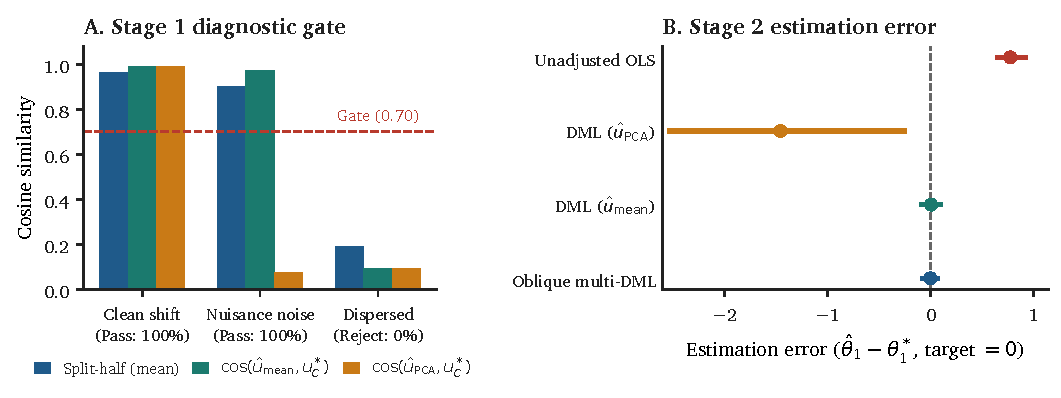
\includegraphics[width=\linewidth]{fig1_simulation}
\caption{Monte Carlo Stage 1 gate diagnostics and Stage 2 estimation error (\simNReps{} replications, $d = \simDim$, $m = \simPairs$, $n = \simObs$). Panel~A compares mean-shift split-half stability and cosine recovery against the $0.70$ rejection threshold across regimes. Panel~B plots mean estimation error $\hat{\theta}_1 - \theta_1^*$ (circles) and 2.5th--97.5th percentile intervals across replications; the dashed line marks zero error.}
\label{fig:simulation}
\end{figure}

In Stage~2, observational representations follow $h_i = C_{1,i} u_{C_1}^* + \nu_i u_{\mathrm{nuis}} + \omega_i u_{\mathrm{conf}} + \epsilon_i$, where $C_{1,i} = 0.8\omega_i + 0.6\nu_i + e_i$ correlates with both the confounder $\omega_i$ and nuisance feature $\nu_i$, and $Y_i = (\simTrueTheta u_{C_1}^* + 1.2 u_{\mathrm{conf}} + 1.0 u_{\mathrm{nuis}})^\top h_i + \xi_i$. For multi-concept estimation, a second concept direction $u_{C_2}^*$ sits at a $45^\circ$ angle to $u_{C_1}^*$ ($\cos\theta = 0.71$) with slope $-1.00$.

Table~\ref{tab:stage2} and Figure~\ref{fig:simulation}B confirm four properties. Unadjusted OLS without $R_i$ suffers severe confounding bias (\simOlsBias, RMSE \simOlsRmse, 0\% coverage). Running DML on the noise-corrupted uncentered PCA direction from the nuisance regime estimates the nuisance slope rather than the concept (bias \simPcaBias). By contrast, 5-fold DML using $\hat{u}_{\mathrm{mean}}$ and the reduced-rank complement $R_{\perp, i}$ achieves near-zero bias (\simMeanBias), low RMSE (\simMeanRmse), and \simMeanCov\% coverage, with healthy overlap $R^2(Z \mid R) = \simMeanRTwo$. Finally, in the multi-concept DGP, applying the naive orthogonal residual formula $(I_d - U_k U_k^\top)h_i$ drives $R^2(Z \mid R) = \simNaiveRTwo$ and causes the estimate to explode (bias \simNaiveBias, RMSE \simNaiveRmse), whereas the oblique pseudoinverse projection~\eqref{eq:oblique} restores clean separation ($R^2 = \simOblRTwo$), near-zero bias (\simOblBias, RMSE \simOblRmse), and \simOblCov\% coverage.

\begin{table}[htbp]
\centering\TableStyle
\caption{Stage 2 causal estimation performance across projection specifications.}
\label{tab:stage2}
\adjustbox{max width=\linewidth}{\begin{tabular}{@{}l rrrr@{}}
\toprule
Estimator / Projection Specification & Bias & RMSE & 95\% Cov. & $R^2(Z \mid R)$ \\
\midrule
Unadjusted OLS (no residual control $R_i$) & +0.773 & 0.776 & 0.000 & 0.00 \\
DML with uncentered PCA $\hat{u}_{\rm PCA}$ (noise-corrupted) & -1.458 & 1.763 & 0.000 & 0.13 \\
DML with mean-shift $\hat{u}_{\rm mean}$ (single concept) & +0.004 & 0.047 & 0.932 & 0.43 \\
Multi-concept DML, naive $U_k^\top h_i$ ($\cos\theta = 0.71$) & +1547.198 & 46245.698 & 1.000 & 1.00 \\
Multi-concept DML, oblique $(U_k^\top U_k)^{-1}U_k^\top h_i$ & -0.002 & 0.037 & 0.938 & 0.16 \\
\bottomrule
\end{tabular}
}
\begin{minipage}{0.95\linewidth}\footnotesize
\emph{Note}: Averages over \simNReps{} replications ($n = \simObs$, true slope $\theta_1^* = \simTrueTheta$, 5-fold cross-fitted DML with ridge nuisance learners on the reduced-rank complement basis $R_{\perp, i}$). 95\% Cov.\ is the empirical coverage of nominal 95\% sandwich intervals. $R^2(Z \mid R)$ is the cross-fitted first-stage overlap diagnostic.
\end{minipage}
\end{table}

\section{Empirical Application: Politeness in Online Requests}

To test the method on real text and human outcomes without a frontier language model, we analyze the Stanford Politeness Corpora \citep{danescu2013computational}: \empNWiki{} Wikipedia talk-page requests and \empNSe{} Stack Exchange technical Q\&A requests, each paired with a crowd-annotated continuous politeness rating (standardized to mean 0, SD 1). As the frozen encoder $h(\cdot)$, we use \texttt{all-MiniLM-L6-v2} (22M parameters, $d = 384$).

\subsection{Stage 1 Diagnostics and Rejection Gate}

External to both corpora, we construct 60 contrastive minimal pairs for politeness across three distinct domains (20 workplace emails, 20 technical queries, 20 everyday requests; examples appear in Appendix~\ref{app:pairs}), converting direct imperatives to polite requests while preserving task content and urgency. To test multi-concept projection and falsification gates, we also construct 60 minimal pairs for urgency, 30 pairs for a negative-control grammatical concept (singular versus plural nouns, which should form a clean linear direction unrelated to politeness), and a sign-flipped placebo formed by randomly multiplying each politeness pair difference by $\pm 1$.

\begin{table}[htbp]
\centering\TableStyle
\caption{Empirical Stage 1 diagnostics on frozen \texttt{all-MiniLM-L6-v2} ($d = 384$).}
\label{tab:emp_stage1}
\adjustbox{max width=\linewidth}{\begin{tabular}{@{}l rrrrc@{}}
\toprule
Concept / Placebo & $R_1^2$ & $\cos(\hat{u}_{\mathrm{PCA}}, \hat{u}_{\mathrm{mean}})$ & Split (Mean) & OOD Transfer & Gate \\
\midrule
Politeness (target, $m=60$) & 0.37 & 0.99 & 0.92 & 0.70 & Pass \\
Urgency (2nd concept, $m=60$) & 0.61 & 1.00 & 0.98 & 0.83 & Pass \\
Plurality (negative control, $m=30$) & 0.30 & 0.99 & 0.84 & -- & Pass \\
Sign-flipped placebo ($m=60$) & 0.37 & 0.58 & 0.14 & 0.13 & Reject \\
\bottomrule
\end{tabular}
}
\begin{minipage}{0.95\linewidth}\footnotesize
\emph{Note}: Computed from external contrastive minimal pairs prior to viewing outcomes. Split (Mean) is the 50-split half-sample cosine of $\hat{u}_{\mathrm{mean}}$. OOD Transfer is the average pairwise cosine across the three pair domains (workplace, technical, everyday); ``--'' denotes a single-domain control set. Gate requires Split (Mean) $\ge 0.70$.
\end{minipage}
\end{table}

Table~\ref{tab:emp_stage1} shows that politeness ($R_1^2 = \empPolROne$, split-half stability \empPolSplit, cross-domain transfer \empPolOod), urgency (split-half \empUrgSplit, transfer \empUrgOod), and the plurality negative control (split-half \empPluSplit) all pass Stage~1. The sign-flipped placebo exhibits the exact same uncentered $R_1^2 = \empRndROne$ as real politeness, confirming that $R_1^2$ alone cannot distinguish a directional concept from zero-mean edit variance. Its mean-shift split-half stability (\empRndSplit) and out-of-domain transfer (\empRndOod), however, collapse and trigger Stage~1 rejection before outcome data are examined.

\subsection{Stage 2 Estimates, Baseline Comparisons, and Placebo Checks}

We project all \empNWiki{} Wikipedia requests and \empNSe{} Stack Exchange requests onto the locked politeness direction $\hat{u}_{\mathrm{mean}}$ (standardized to 1-SD units) and run 5-fold cross-fitted DML with cross-validated ridge regression on $R_{\perp, i} \in \mathbb{R}^{383}$. Table~\ref{tab:emp_stage2} and Figure~\ref{fig:empirical} report the main estimates, comparisons against three standard baselines, and three Stage~2 placebo suites.

\begin{figure}[htbp]
\centering
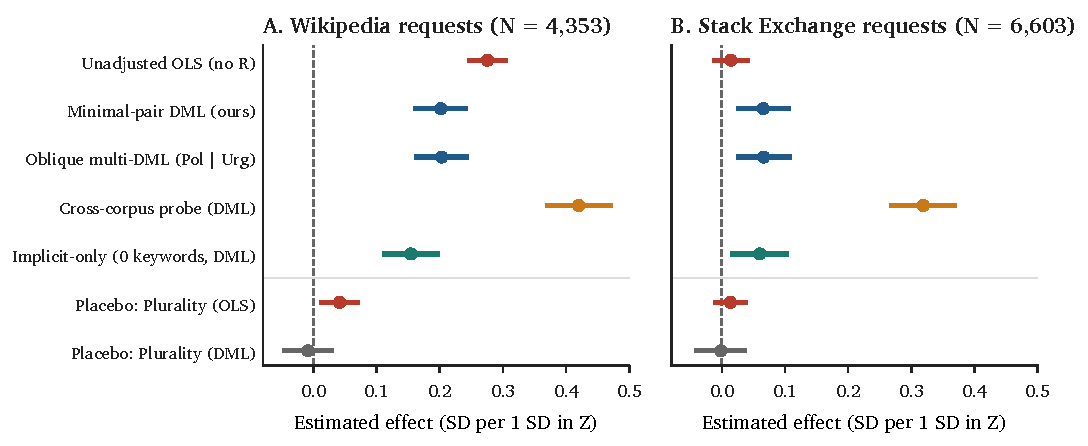
\includegraphics[width=\linewidth]{fig2_empirical}
\caption{Empirical Stage 2 politeness estimates, baseline comparisons, and negative-control placebos across Wikipedia ($N = \empNWiki$) and Stack Exchange ($N = \empNSe$) requests on frozen \texttt{all-MiniLM-L6-v2}. Circles show point estimates in outcome SD per 1-SD shift in $Z$; bars show 95\% sandwich confidence intervals. The horizontal rule separates target and baseline specifications from the plurality negative-control placebo; the vertical dashed line marks zero.}
\label{fig:empirical}
\end{figure}

\begin{table}[htbp]
\centering\TableStyle
\caption{Empirical Stage 2 estimates, baseline comparisons, and placebo checks.}
\label{tab:emp_stage2}
\adjustbox{max width=\linewidth}{\begin{tabular}{@{}l r r r r@{}}
\toprule
 & \multicolumn{2}{c}{Wikipedia ($N=4{,}353$)} & \multicolumn{2}{c}{Stack Exchange ($N=6{,}603$)} \\
\cmidrule(lr){2-3} \cmidrule(lr){4-5}
Specification / Placebo Check & $\hat{\theta}$ (SE) & $R^2(Z{\mid}R)$ & $\hat{\theta}$ (SE) & $R^2(Z{\mid}R)$ \\
\midrule
\multicolumn{5}{@{}l}{\emph{Panel A: Target Concept (Politeness, 1 SD)}} \\
Unadjusted OLS (no $R_i$ control) & +0.275 (0.014) & -- & +0.014 (0.013) & -- \\
5-fold DML (minimal-pair $\hat{u}_{\mathrm{mean}}$) & +0.202 (0.020) & 0.64 & +0.065 (0.020) & 0.62 \\
Oblique Multi-DML (Politeness $|$ Urgency) & +0.203 (0.020) & 0.63 & +0.066 (0.020) & 0.62 \\
Naive Multi-DML (broken $U_k^\top h_i$) & +1.900 (0.232) & 1.00 & +0.853 (0.305) & 1.00 \\
\midrule
\multicolumn{5}{@{}l}{\emph{Panel B: Comparisons Against Baselines}} \\
Cross-corpus supervised probe (DML) & +0.420 (0.025) & 0.76 & +0.319 (0.025) & 0.74 \\
Implicit-only subset (0 keywords; ours) & +0.154 (0.021) & 0.62 & +0.060 (0.022) & 0.63 \\
\midrule
\multicolumn{5}{@{}l}{\emph{Panel C: Placebo Checks (Expected Null)}} \\
Negative-control concept: Plurality (OLS) & +0.041 (0.015) & -- & +0.014 (0.012) & -- \\
Negative-control concept: Plurality (DML) & -0.009 (0.019) & 0.61 & -0.002 (0.019) & 0.61 \\
Outcome permutations (20$\times$, reject@5\%) & 0.0\% & -- & 0.0\% & -- \\
Random $\perp$ directions (20$\times$, OLS reject@5\%) & 70.0\% & -- & 50.0\% & -- \\
Random $\perp$ directions (20$\times$, DML reject@5\%) & 5.0\% & -- & 5.0\% & -- \\
\bottomrule
\end{tabular}
}
\begin{minipage}{0.95\linewidth}\footnotesize
\emph{Note}: Outcome is the standardized human politeness rating (mean 0, SD 1); treatment coordinates $Z$ are standardized to 1-SD units. Heteroskedasticity-robust sandwich standard errors appear in parentheses. ``--'' denotes unadjusted OLS or permutation/random-direction rejection rates where first-stage $R^2(Z \mid R)$ is not applicable. Implicit-only rows restrict to the \empWikiNoKwN{} Wikipedia (\empWikiNoKwPct\%) and \empSeNoKwN{} Stack Exchange (\empSeNoKwPct\%) requests containing zero explicit politeness keywords.
\end{minipage}
\end{table}

Confounding adjustment matters in opposite directions across the two corpora (Table~\ref{tab:emp_stage2}, Panel~A). On Wikipedia, unadjusted OLS overstates the politeness slope (\empWikiOls{} versus \empWikiDml{}, SE \empWikiDmlSe{} under 5-fold DML). On Stack Exchange, technical-topic confounding suppresses unadjusted OLS to near zero (\empSeOls, SE \empSeOlsSe), whereas controlling for $R_{\perp, i}$ recovers a positive politeness effect of \empSeDml{} (SE \empSeDmlSe). Proposition~\ref{prop:oblique} also appears directly in real text: although politeness and urgency share only a modest cosine overlap (\empCosPolUrg), applying the naive orthogonal residual $(I_d - U_2 U_2^\top)h_i$ drives $R^2(Z_1 \mid R)$ to $1.00$ and inflates the politeness estimate to \empWikiNav{} on Wikipedia and \empSeNav{} on Stack Exchange. Switching to the oblique pseudoinverse projection restores healthy overlap ($R^2 = \empWikiRTwo$ and \empSeRTwo) and exact recovery (\empWikiObl{} and \empSeObl).

Comparing our design against three standard baselines clarifies its practical advantages and tradeoffs (Panel~B). Explicit politeness keywords (\texttt{please}, \texttt{thank}, \texttt{could you}, \texttt{would you}, \texttt{kindly}, \texttt{appreciate}) are absent from \empWikiNoKwPct\% of Wikipedia requests (\empWikiNoKwN{} texts) and \empSeNoKwPct\% of Stack Exchange requests (\empSeNoKwN{} texts), leaving lexical proxies undefined on most of both corpora. Restricted to those zero-keyword requests, our minimal-pair subspace DML still detects implicit politeness effects of \empWikiImp{} (SE \empWikiImpSe) on Wikipedia and \empSeImp{} (SE \empSeImpSe) on Stack Exchange. Unsupervised latent discovery fares worse still: the top principal component of observational embeddings achieves only \empPcPairAcc\% directional accuracy on controlled minimal pairs (worse than chance) and primarily tracks corpus domain ($|r| = \empPcDomR$). Finally, training a cross-corpus supervised ridge probe on the opposite corpus yields larger DML slopes (\empWikiProbe{} on Wikipedia and \empSeProbe{} on Stack Exchange) because it fits the broader Stanford annotation rubric using thousands of labeled outcomes. That extra predictive power comes with a clear cost: the observational probe requires \empNWiki{} to \empNSe{} human-labeled training outcomes (versus zero outcome labels in our Stage~1), absorbs four to five times more text-length correlation ($|r| = \empRLenProbeLo$ to \empRLenProbeHi{} versus \empRLenOurs{} for our minimal-pair direction), and exhibits stronger entanglement with background representations ($R^2(Z \mid R) = \empSeProbeRTwo$ to \empWikiProbeRTwo{} versus \empSeRTwo{} to \empWikiRTwo), inflating DML standard errors by 25\%.

All three Stage~2 placebo suites validate the DML specification (Panel~C). For the negative-control plurality direction, which passed Stage~1, unadjusted OLS produces a spurious positive effect on Wikipedia (\empWikiPluOls, SE \empWikiPluOlsSe), whereas 5-fold DML returns a clean null on both corpora (\empWikiPluDml{} and \empSePluDml, SE \empWikiPluDmlSe). Across 20 random outcome permutations, DML rejects 0.0\% of the time. Across 20 random unit directions orthogonal to politeness, unadjusted OLS suffers severe false-positive inflation, rejecting \empWikiRandOls\% on Wikipedia and \empSeRandOls\% on Stack Exchange at the 5\% level due to representation anisotropy, while 5-fold DML achieves exact \empWikiRandDml\% nominal rejection on both corpora.

\section{Discussion}

Three practical choices govern how well subspace-constrained causal inference works in applied research. First, layer selection belongs strictly inside Stage~1. Abstract semantic and stylistic concepts tend to separate most linearly in middle-to-late transformer layers rather than the token-embedding layer or the final next-token prediction head \citep{alain2016understanding,zou2023representation}. Researchers should evaluate Stage~1 diagnostics across candidate layers using only $\mathcal{D}_{\mathrm{pairs}}$ and lock the layer before touching outcomes; choosing a layer to maximize a Stage~2 $t$-statistic invalidates inference.

Second, not every concept forms a global linear subspace. When split-half stability passes within domains but out-of-domain transfer fails across domains, the concept acts along different directions in different contexts, and researchers should estimate domain-stratified subspaces $U_k^{(g)}$. Where concepts are sparse or polysemantic in the residual stream, our two-stage logic extends directly to overcomplete dictionary features from sparse autoencoders \citep{cunningham2023sparse}: minimal pairs test whether concept $C$ concentrates on a small set of dictionary features in Stage~1, and Stage~2 controls for the remaining active features.

Third, the framework makes its identifying assumptions explicit and partially testable, but it does not eliminate observational confounding outside the text. If an unobserved external variable (such as author prestige not encoded in $T_i$) drives both $Z_i$ and $Y_i$, controlling for $R_{\perp, i}$ cannot remove that bias. Even within the text, the resulting estimand is a local, representation-dependent causal effect along the locked subspace $\hat{U}_k$. Pairing minimal-pair Stage~1 gates with round-trip decoding checks in experiments, or reduced-rank DML and placebo suites in observational corpora, gives applied researchers a disciplined way to isolate one concept at a time and a clear rule for stopping when the representation cannot support the question.

\bibliographystyle{working-paper-apsr}
\bibliography{references}

\appendix

\section{Proofs}\label{app:proofs}

\begin{proof}[Proof of Proposition~\ref{prop:oblique}]
For any $h_i \in \mathbb{R}^d$, decomposing $h_i = U_k Z_i + R_i$ with $U_k^\top R_i = 0$ requires $U_k^\top h_i = (U_k^\top U_k)Z_i + U_k^\top R_i = G_k Z_i$. Because $\mathrm{rank}(U_k) = k$, $G_k$ is symmetric positive definite and invertible, yielding $Z_i = G_k^{-1}U_k^\top h_i$ and $R_i = h_i - U_k Z_i = (I_d - U_k G_k^{-1} U_k^\top)h_i$. Pre-multiplying by $U_k^\top$ verifies $U_k^\top R_i = U_k^\top h_i - G_k G_k^{-1}U_k^\top h_i = 0$, and substituting $h_i = U_k Z_i^* + R_i^*$ with $U_k^\top R_i^* = 0$ gives $Z_i = G_k^{-1}G_k Z_i^* = Z_i^*$. By contrast, under the naive formula $R_i^{\mathrm{naive}} = (I_d - U_k U_k^\top)h_i$, pre-multiplying by $U_k^\top$ gives $U_k^\top R_i^{\mathrm{naive}} = (I_k - G_k)U_k^\top h_i$, which vanishes for all $h_i$ if and only if $G_k = I_k$. When $G_k \neq I_k$, $(I_k - G_k)U_k^\top h_i$ is an invertible linear function of $Z_i^*$ in the absence of noise, so $Z_i^{\mathrm{naive}}$ lies in the linear span of $R_i^{\mathrm{naive}}$ and $R^2(Z^{\mathrm{naive}} \mid R^{\mathrm{naive}}) \to 1$.
\end{proof}

\begin{proof}[Proof of Proposition~\ref{prop:inference}]
For part~(a), independence $\mathcal{D}_{\mathrm{pairs}} \perp \mathcal{D}_{\mathrm{obs}}$ implies that conditional on $\mathcal{D}_{\mathrm{pairs}}$, the matrix $\hat{U}_k$ and any orthonormal complement basis $\hat{U}_\perp$ are non-random, and the observations $\{(Y_i, Z_i(\hat{U}_k), R_{\perp, i}(\hat{U}_k))\}_{i=1}^n$ remain i.i.d.\ draws from the conditional law given $\mathcal{D}_{\mathrm{pairs}}$. Applying Theorem~4.1 of \citet{chernozhukov2018double} conditional on $\mathcal{D}_{\mathrm{pairs}}$ yields~\eqref{eq:dml} and asymptotic normality centered at $\theta_0(\hat{U}_k)$.

For part~(b), under Equation~\eqref{eq:edit_model} with $k = 1$, $\bar{\Delta h} = \mu_\alpha u_C^* + \bar{\varepsilon}$ where $\bar{\varepsilon} = O_P(m^{-1/2})$, so normalizing yields $\|\hat{u}_{\mathrm{mean}} - u_C^*\|_2 = O_P(m^{-1/2}/|\mu_\alpha|)$. For a $k$-dimensional eigenspace of a symmetric matrix estimator $\hat{M}$ satisfying $\|\hat{M} - M\|_{\mathrm{op}} = O_P(m^{-1/2})$ with population eigengap $\delta_k = \lambda_k - \lambda_{k+1} > 0$, the Davis--Kahan $\sin\Theta$ theorem \citep{davis1970rotation} yields $\|P_{\hat{U}_k} - P_{U_k^*}\|_{\mathrm{op}} \le 2\|\hat{M} - M\|_{\mathrm{op}}/\delta_k = O_P(m^{-1/2}/\delta_k)$. Since $\theta_0(\hat{u}_C) - \theta_0(u_C^*) = \beta_h^\top(\hat{u}_C - u_C^*) + O_P(\|\hat{u}_C - u_C^*\|_2)$ under bounded $\|\beta_h\|_2$, the bias between the locked-subspace estimand and the population subspace estimand is $O_P(m^{-1/2}/\delta_k)$, which is $o_P(n^{-1/2})$ whenever $\sqrt{n}/(m^{1/2}\delta_k) \to 0$.
\end{proof}

\section{External Minimal-Pair Examples}\label{app:pairs}

Table~\ref{tab:pairs_examples} lists representative external minimal pairs from the three domains used in Stage~1 of the empirical application. All 60 politeness pairs, 60 urgency pairs, and 30 plurality pairs are published in the replication script \texttt{scripts/empirical\_politeness.py}.

\begin{table}[htbp]
\centering\TableStyle
\caption{Representative external minimal pairs used in Stage 1.}
\label{tab:pairs_examples}
\adjustbox{max width=\linewidth}{\begin{tabular}{@{}l p{5.5cm} p{6.2cm}@{}}
\toprule
Concept (Domain) & Baseline ($T_j^-$) & Contrastive Edit ($T_j^+$) \\
\midrule
Politeness (Workplace) & Send me the quarterly budget spreadsheet by Friday. & Could you please send me the quarterly budget spreadsheet by Friday? \\
Politeness (Technical) & Explain why this SQL query returns duplicate rows. & Would you mind explaining why this SQL query returns duplicates? \\
Politeness (Everyday) & Hold the elevator door for a second. & Would you mind holding the elevator door for a second? \\
Urgency (Workplace) & Send me the quarterly budget spreadsheet by Friday. & Send me the quarterly budget spreadsheet by Friday immediately, this is urgent. \\
Plurality (Control) & I checked the report on the desk. & I checked the reports on desks. \\
\bottomrule
\end{tabular}
}
\begin{minipage}{0.95\linewidth}\footnotesize
\emph{Note}: Representative pairs from the external minimal-pair corpus constructed independently of the Wikipedia and Stack Exchange datasets. All 60 politeness pairs, 60 urgency pairs, and 30 plurality pairs are in \texttt{scripts/empirical\_politeness.py}.
\end{minipage}
\end{table}

\end{document}
